
\documentclass{article}

\usepackage{minted}
\usepackage{graphicx}


\begin{document}

\title{Evolutionary Algorithms - Project Report }
\author{EL KHADIR Bachir \\
Ecole Polytechnique}
\date{\today}
\maketitle


\begin{abstract}
This paper presents the result ...
I choose \textit{Python} as a programming langage.
\end{abstract}

\section{Implementation of the GA algorithm}
The EA class implmenets the $(1+(\lambda, \lambda))$ GA in a generic form. The constructor is:
\mint{python}|def __init__(self, fitness, mutation=None, crossover=None)|
It requires:
\begin{itemize}
	\item a fitness function to evaluate individuals,
	\item a mutation operator, by default, this operator is used:
\begin{minted}{python}
	def default_mutation(l, x):
		bits_to_change 	= random.sample(range(len(x)), l)
		x_mut 					= list(x)
		for b in bits_to_change:
				x_mut[b] = random.choice([0, 1])
		return x_mut
\end{minted}
	\item a crossover operator
\begin{minted}{python}
	def default_crossover(c, x, xx):
			parent 				= [x, xx]
			parent_choice = bernoulli.rvs(c, size=len(x))
			return [ parent[p][i] for i, p in enumerate(parent_choice) ]
\end{minted}
		
\end{itemize}

Then, the \textit{run} function /* bla bla bla */
\mint{python}|def run(self, n, x_init, offspring_size=5, n_generations=10, p=None, c=None, self_adapt=False, max_fitness=None)|

\subsection{The One-Max problem}
The implmentation of the one-max problem is straight forward. 
We start with a random vector in ${0, 1}^n$. Default mutation and crossover operator work fine. 
For the fitness function, we sum up all the bits in x (there is a builtin function \textit{sum} provided with \textit{Python}). The code is as follow:
\begin{minted}{python}
ea_algo = ga.EA(fitness=sum)
x_init 	= np.random.random_integers(0, 1, size=n)
best_x 	= ea_algo.run(n, x_init, offspring_size=5, n_generations=100)
\end{minted}

\textbf{Self adaptative rule}

\subsection{The Maximum Matching}
We represent an undirected graph like suggested in the **** Feuille de projet ****. For example:

\begin{minted}{python}
vertices = range(n)
edges = [(i, i+1) if i+1 < n else (n-1, 0) for i in range(n)]
\end{minted}

The function reponsible for calculating the degree of a vertex $v$ in ine the subgraph consisting of the edges of $M$:
\begin{minted}{python}
def deg(M):
    deg_m = np.zeros(m)
    for i, (e, f) in enumerate(edges):
        if M[i]:
            deg_m[e] += 1
            deg_m[f] += 1
    return sum([max(0, d-1) for d in deg_m])
\end{minted}

And the fitness function:

\begin{minted}{python}
def fitness(M): 
    return sum(M) - m * deg(M)
\end{minted}

Here is the result (edges of the best matching are coloured in red):\\
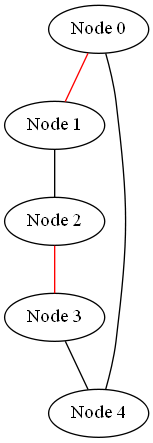
\includegraphics[scale=0.5]{img/max_graph.png}

\subsection{Euler cycles}

\end{document}
